\documentclass[border=196pt]{standalone}
\usepackage{tikz}

\begin{document}
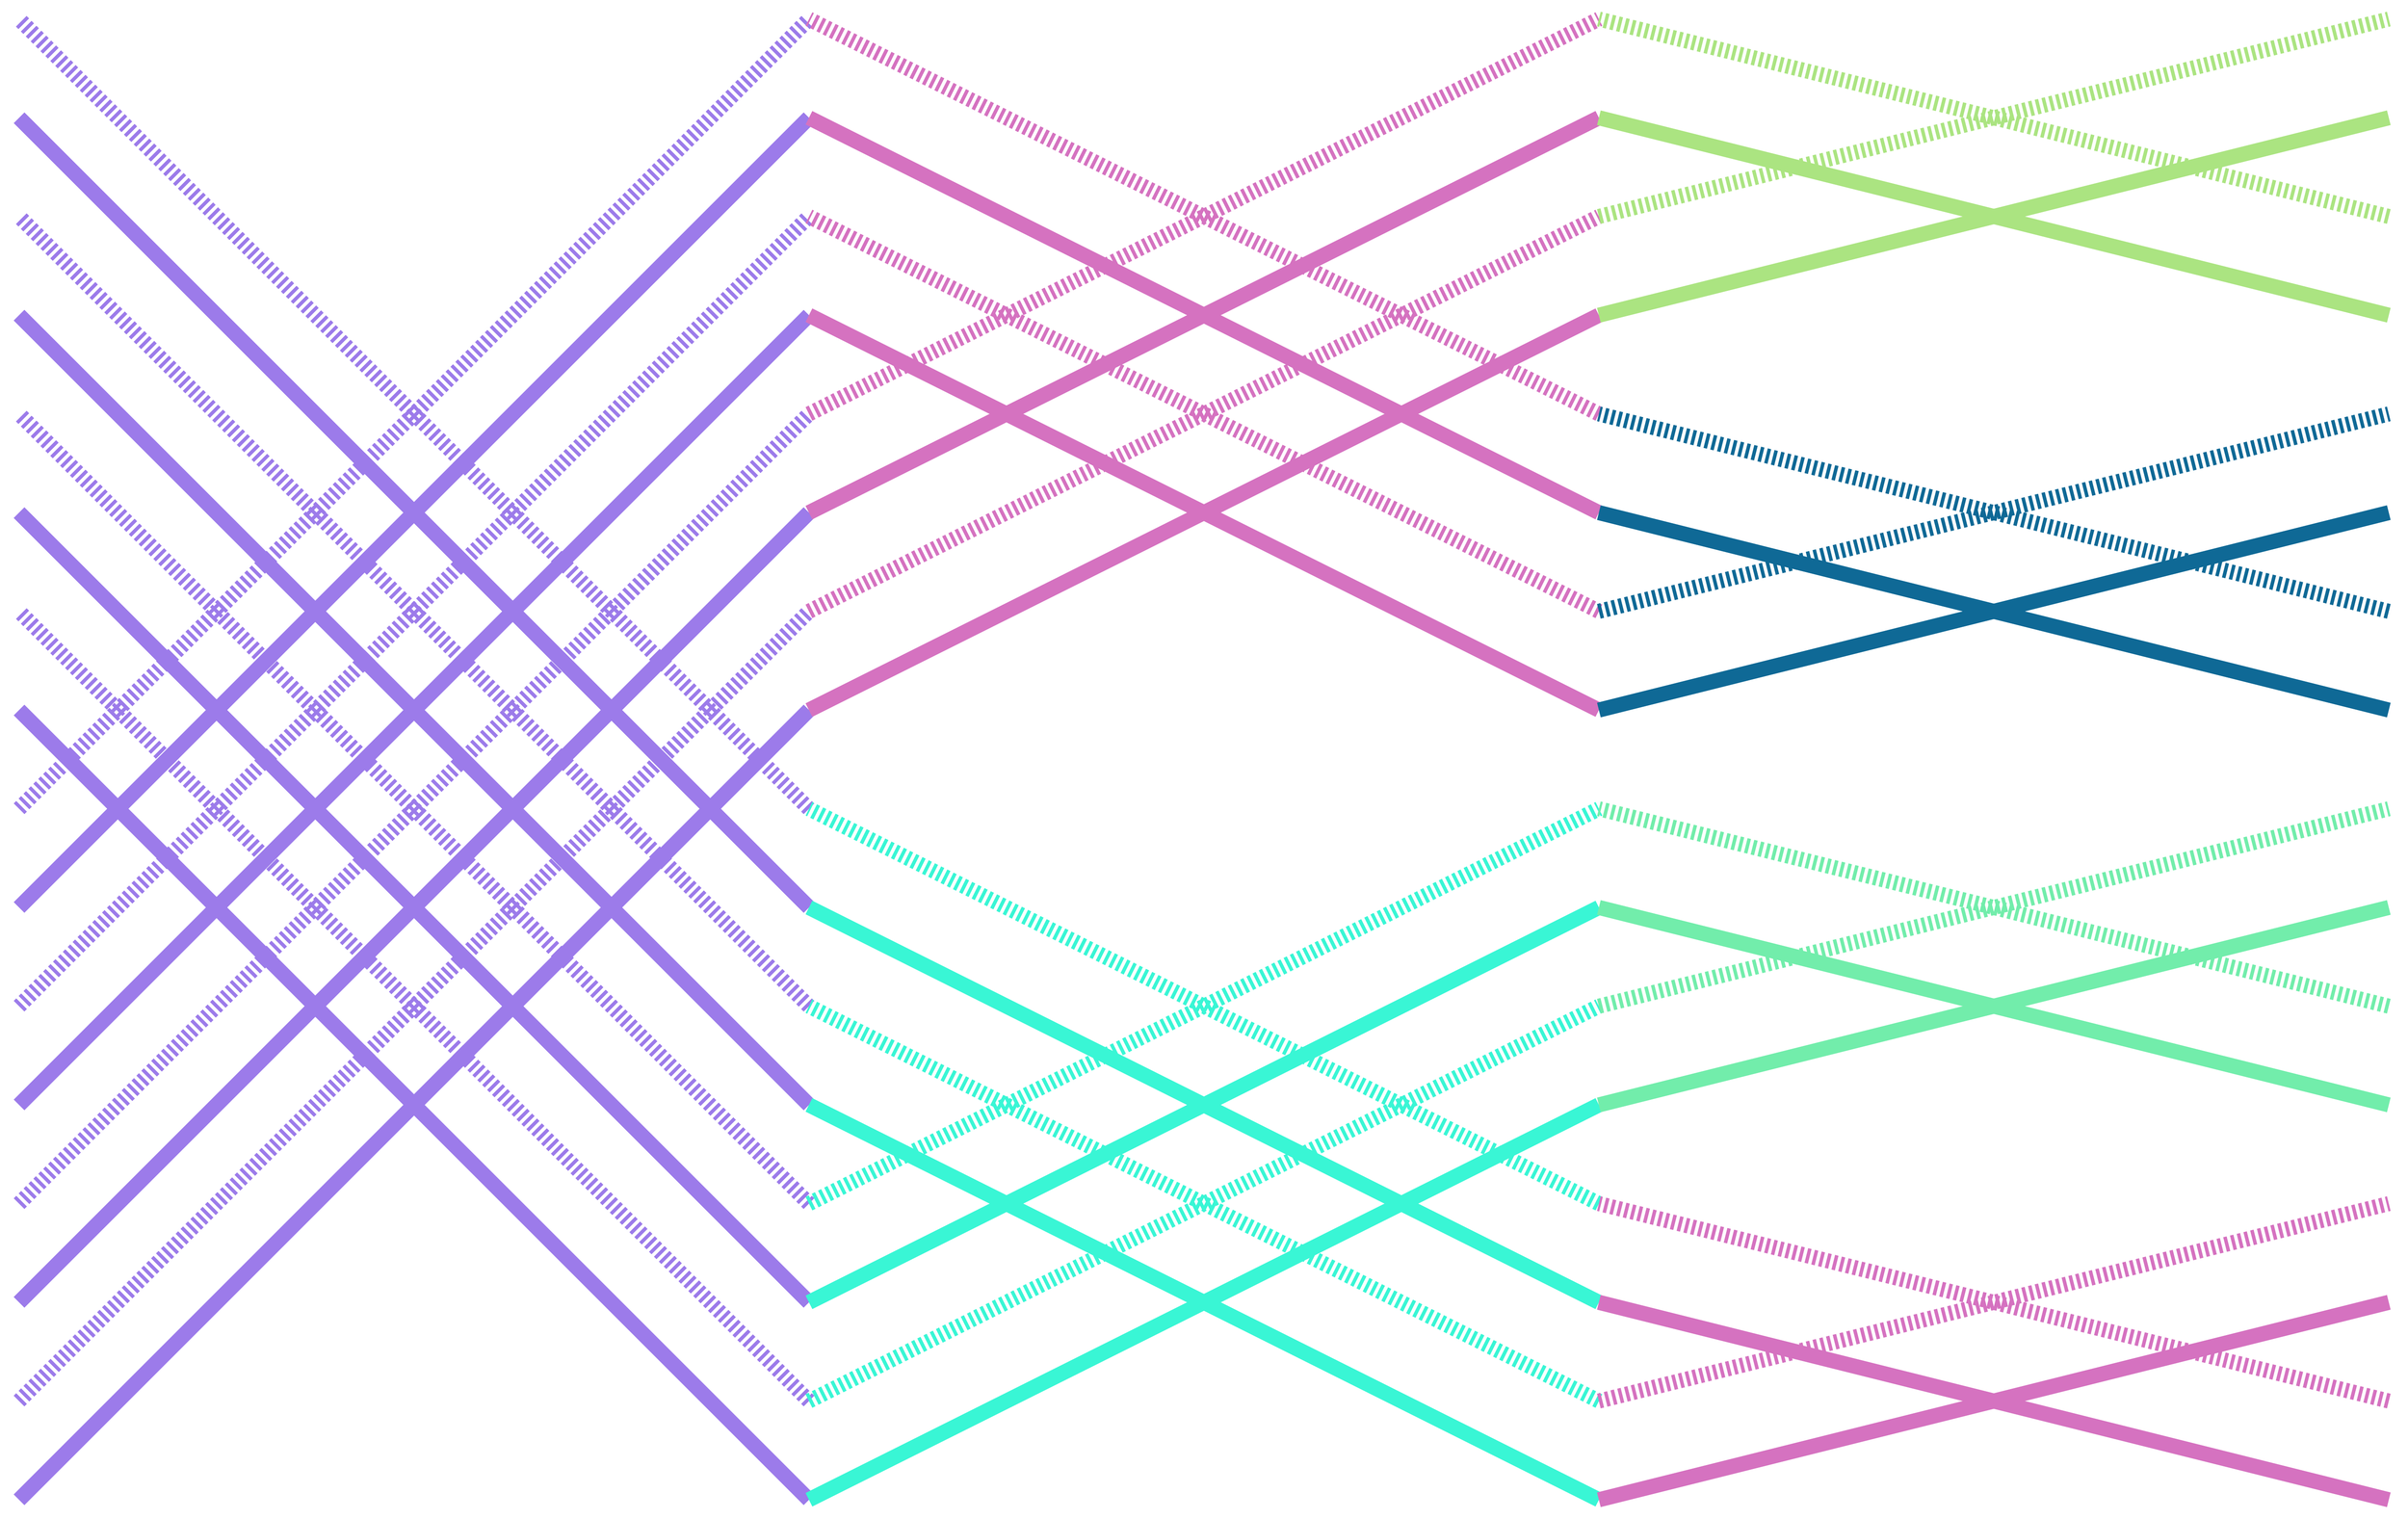
\begin{tikzpicture}

  \pgfmathtruncatemacro\xrange{4}
  \pgfmathtruncatemacro\yrange{2^\xrange-1}
  \foreach \x in {0,...,\xrange}
    \foreach \y in {0,...,\yrange} 
      \coordinate (\x\y) at (24*\x,3*\y) {};
 
  \pgfmathtruncatemacro\levelrange{\xrange-2}
  \foreach \level in {0,...,\levelrange}
  {
    \pgfmathtruncatemacro\nextlevel{\level+1}
    \pgfmathtruncatemacro\step{2^(\xrange-1-\level)}
    \pgfmathtruncatemacro\startrange{2^(\xrange-1)/\step-1}
    \foreach \startcount in {0,...,\startrange} 
      {
        \pgfmathtruncatemacro{\start}{\startcount*\step*2}
        \pgfmathtruncatemacro{\startplustwo}{\start+2}
        \pgfmathtruncatemacro{\lrange}{\start+\step-1}
        \pgfmathtruncatemacro{\lcntstart}{\start/2}
        \pgfmathtruncatemacro{\lcntend}{\lrange/2}
        \foreach \lcnt in {\lcntstart,...,\lcntend}
        {
          \pgfmathtruncatemacro{\l}{\lcnt*2}
          \pgfmathtruncatemacro{\h}{\l+\step}
          \pgfmathtruncatemacro{\cr}{{Mod((\startcount+\level+1)*666, 255)}}
          \pgfmathtruncatemacro{\cg}{{Mod((\startcount+\level+1)*888, 255)}}
          \pgfmathtruncatemacro{\cb}{{Mod((\startcount+\level+1)*999, 255)}}
          \definecolor{currentColor}{RGB}{\cr,\cg,\cb};
          \draw [currentColor, line width = 13] (\level\l) -- (\nextlevel\h);
          \draw [currentColor, line width = 13] (\nextlevel\l) -- (\level\h);
        }
        \foreach \lcnt in {\lcntstart,...,\lcntend}
        {
          \pgfmathtruncatemacro{\l}{\lcnt*2+1}
          \pgfmathtruncatemacro{\h}{\l+\step}
          \pgfmathtruncatemacro{\cr}{{Mod((\startcount+\level+1)*666, 255)}}
          \pgfmathtruncatemacro{\cg}{{Mod((\startcount+\level+1)*888, 255)}}
          \pgfmathtruncatemacro{\cb}{{Mod((\startcount+\level+1)*999, 255)}}
          \definecolor{currentColor}{RGB}{\cr,\cg,\cb};
          \draw [currentColor, line width = 13, dashed] (\level\l) -- (\nextlevel\h);
          \draw [currentColor, line width = 13, dashed] (\nextlevel\l) -- (\level\h);
        }
      } 
  }

\end{tikzpicture}
\end{document}  